\documentclass{article}
\usepackage{graphicx}
\usepackage{caption}
\usepackage{subcaption}
\usepackage{url}

\usepackage{amsmath}

\newcommand{\code}[1]{\texttt{#1}}
\renewcommand\refname{7  \hspace{4 mm}References}

\begin{document}

\title{CS 867: Displaying Multiple Time Series}
\date{December 16, 2013}
\author{Carmen St.\ Jean}

\maketitle

\section{Introduction}

Time-oriented data might be one of the most common forms of data, used in numerous fields such as medicine, economics, ecology, engineering, and meteorology.  Typically, time series are visualized using line charts, which appear frequently in newspapers, textbooks, and academic papers.  However, it can be difficult to display many concurrent time series at once in an understandable manner using a line chart.  Therefore, we have introduced a new visualization technique called a stack graph, which we propose may be suitable for showing many time series---i.e., fifteen---at once.  To test the merits of our creation, we have evaluated the stacked graph against two existing methods---small multiples and horizon graphs.

\subsection{Background}

Since it was first introduced by William Playfair in 1786 \cite{playfair1786}, the line chart has been a popular choice for displaying temporal data.  However, it has its limitations when it comes to multiple time series.  To be plotted on a single chart, each time series must be distinctly colored and/or patterned; as the number of time series increases, it becomes more difficult to make each series visually distinct.  Even if each time series are designed uniquely, it may be difficult to distinguish two time series which overlap frequently.

\begin{figure}
        \centering
        \begin{subfigure}[b]{0.4\textwidth}
                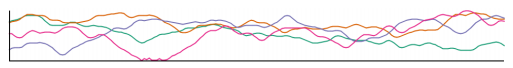
\includegraphics[width=\textwidth]{figures/ts_simplelinegraph.png}
                \caption{A simple line graph.}
                \label{fig:ts_simple}
        \end{subfigure}
        \begin{subfigure}[b]{0.4\textwidth}
                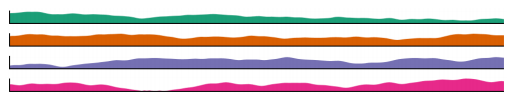
\includegraphics[width=\textwidth]{figures/ts_smallmultiples.png}
                \caption{Small multiples.}
                \label{fig:ts_smmult}
        \end{subfigure}
        \\
        \begin{subfigure}[b]{0.4\textwidth}
                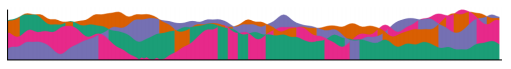
\includegraphics[width=\textwidth]{figures/ts_braidedgraph.png}
                \caption{A braided graph.}
                \label{fig:ts_braid}
        \end{subfigure}
        \begin{subfigure}[b]{0.4\textwidth}
                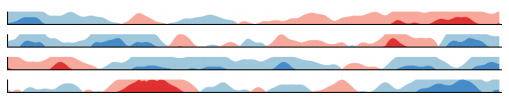
\includegraphics[width=\textwidth]{figures/ts_horizongraphs.png}
                \caption{Horizon graphs.}
                \label{fig:ts_horizon}
        \end{subfigure}
        \caption{Four possible methods for visualizing multiple time series \cite{javed2010}.}
        \label{fig:ts_compare}
\end{figure}

Recognizing the limitations of the line chart for many time series leads to a question: what is a suitable alternative?  Javed et al.\ set out to answer this question with their evaluation that compared the line chart, as in Figure~\ref{fig:ts_simple}, with three alternative techniques  \cite{javed2010}.  The first alternative, called ``small multiples'' simply places each time series on its own line chart, shown in Figure~\ref{fig:ts_smmult}.  The screen space must be split with this approach, which leads to less resolution in the vertical direction.  Therefore, Javed et al.\ introduced a shared space approach called the ``braided graph'' seen in Figure~\ref{fig:ts_braid}, which attempts to be easier to read than a line chart by coloring the areas underneath the curves.  Additionally, Saito et al.'s horizon graph, as in Figure~\ref{fig:ts_horizon}, was included in the evaluation \cite{saito2005}.

\begin{figure}
        \centering
        \begin{subfigure}[b]{0.5\textwidth}
                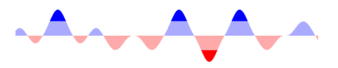
\includegraphics[width=\textwidth]{figures/construction1.png}
                \caption{The line chart is divided into evenly-spaced bands, which are colored shades of blue in the upper-half and shades of red in the lower-half.}
                \label{fig:construction1}
        \end{subfigure}
        \\ 
        \begin{subfigure}[b]{0.5\textwidth}
                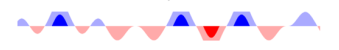
\includegraphics[width=\textwidth]{figures/construction2.png}
                \caption{The bands of similar colors are layered together.}
                \label{fig:construction2}
        \end{subfigure}
        \\
        \begin{subfigure}[b]{0.5\textwidth}
                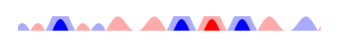
\includegraphics[width=\textwidth]{figures/construction3.png}
                \caption{The red bands are mirrored.}
                \label{fig:construction3}
        \end{subfigure}
        \caption{Four possible methods for visualizing multiple time series \cite{javed2010}.}
        \label{fig:hg_construction}
\end{figure}

Saito et al.\ designed horizon graphs to increase the amount of data that can be displayed without increasing graph size \cite{saito2005}.  To construct a horizon graph, some ``mid-line'' must be defined; it could represent zero or it could be the average of the global minimum and global maximum values in the dataset.  The areas between the mid-line and the data values are filled in, as in Figure~\ref{fig:construction1}, with blue for areas above the mid-line and red for areas below the mid-line.  The data is then further divided into evenly spaced bands, with the color of the band darkening as distance from the mid-line increases.  Next, these bands are offset to align with the mid-line, as in Figure~\ref{fig:construction2}.  Finally, the red bands are mirrored.  The result is the vertical resolution can be increased by a factor of four, as in Figure~\ref{fig:hg_construction}, or even more if more bands are used.

Javed et al.\ evaluated these four techniques illustrated in Figure~\ref{fig:ts_compare} by having participants complete three tasks on randomly-generated data:
\begin{enumerate}
	\item \textbf{Maximum:} for a given time point, identify the time series with the highest value
	\item \textbf{Slope:} for the entire time period, find the time series with the highest increase
	\item \textbf{Discrimination:} at a time point specific to each series, determine which series has the highest values
\end{enumerate}
In addition to chart type, their study varied the number of time series (2, 4, and 8) and the total chart height (48, 96, and 192 pixels).  They found that the simple line chart and the braided graph were best suited for the maximum task, while the small multiples and horizon graphs were better for the slope and discrimination tasks.  In general, they concluded that simple line charts and small multiples were generally more robust than horizon graphs and their newly introduced braided graphs. Additionally, they found that decreases in chart size did not affect completion time, but did decrease accuracy.  Lastly, as the number of concurrent time series increased, accuracy decreased and completion time increased. 

\bibliographystyle{plain}

\bibliography{sources}

\end{document}